\documentclass[]{article}

\usepackage{graphicx}

\usepackage[margin=1in]{geometry}

\setlength\parindent{0pt}

\usepackage{physics}
\usepackage{amsmath}
\usepackage{amsfonts}
\usepackage{amssymb}

\usepackage{listings}

\usepackage{enumitem}
\renewcommand{\theenumi}{\alph{enumi}}
\renewcommand*{\thesection}{Problem \arabic{section}}
\renewcommand*{\thesubsection}{\arabic{section}\alph{subsection})}
\renewcommand*{\thesubsubsection}{\quad \roman{subsubsection})}

%Custom Commands
\newcommand{\Rel}{\mathcal{R}}
\newcommand{\R}{\mathbb{R}}
\newcommand{\C}{\mathbb{C}}
\newcommand{\N}{\mathbb{N}}
\newcommand{\Z}{\mathbb{Z}}
\newcommand{\Q}{\mathbb{Q}}

\newcommand{\toI}{\xrightarrow{\textsf{\tiny I}}}
\newcommand{\toS}{\xrightarrow{\textsf{\tiny S}}}
\newcommand{\toB}{\xrightarrow{\textsf{\tiny B}}}

\newcommand{\divisible}{ \ \vdots \ }


%opening

\title{MATH 5301 Elementary Analysis - Homework 3}

\author{Jonas Wagner}

\date{2021, September 17}



\begin{document}

\maketitle

% Problem 1
\section{}
Let $X$ denote the universal set. Two subsets $A$ and $B$ are said to have 
the same cardinality if there is a bijection $f : A \to B$.
Notation: $\abs*{A} = \abs*{B}$.

\subsection{
	Prove that $\abs{A} = \abs{B}$ is an equivalence relation on the power set of $X$
}

The relation $\Rel = ``\abs{A} = \abs{B}''$
\footnote{using $\Rel$ for simplicyity/reusability} 
is defined as: 
$$\Rel = ``\abs{A} = \abs{B}'' = \{(A,B) : \exists (f : A \xrightarrow{\textsf{\tiny B}} B)\}$$

Equivilence can be demonstrated by proven by demonstrating: 
(i) Reflexivity, (ii) Symetry, and (iii) Transivity


\subsubsection{Reflective:}
\begin{align*}
	A \Rel A
		&= \{(A,A) : \exists (f : A \toB A)\}
\end{align*}
Since $f : A \toB A = {a \in A}$ is true $\forall A \in 2^X$, $\R$ is Reflective.

\subsubsection{Symetric:}
\begin{align*}
	A \Rel B 
		&\implies B \Rel A\\
	\{(A,B) : \exists (f : A \xrightarrow{\textsf{\tiny B}} B)\}
		&\implies \{(B,A) : \exists (f : B \xrightarrow{\textsf{\tiny B}} A)\}
\end{align*}
Since $f : A \toB B \implies g : B \toB A = f^{-1}$ is true $\forall A,B \in 2^X$, 
$\R$ is Symetric.\\
(Essentially if $f$ is bijective one way, 
$f^{-1}$ is bijective for the other way)

\subsubsection{Transative:}
\begin{align*}
	(A \Rel B) 
		\land (B \Rel C) 
		&\implies A \Rel C\\
	(\{(A,B) : \exists (f : A \xrightarrow{\textsf{\tiny B}} B)\})
		\land \{(B,C) : \exists (g : B \xrightarrow{\textsf{\tiny B}} C)\}
		&\implies \{(A,C) : \exists (h : A \xrightarrow{\textsf{\tiny B}} C)\}
\end{align*}
Since $(f : A \toB B) \land (g : B \toB C) 
\implies (h : A \toB C = A \xrightarrow{f} B \xrightarrow{g} C)$ 
is true $\forall A,B,C \in 2^X$, $\Rel$ is Transative.\\

Therefore $\Rel = ``\abs{A} = \abs{B}''$ is an equivalence relation over $2^X$.

\newpage
\subsection{
	Is it true that if $\abs{A_1}=\abs{B_1}$ and $\abs{A_2}=\abs{B_2}$ 
	then $\abs{A_1 \cup A_2} = \abs{B_1 \cup B_2}$?
}
\begin{align*}
	(\abs{A_1} = \abs{B_1}) \land (\abs{A_2} = \abs{B_2})
		&\implies \abs{A_1 \cup A_2} = \abs{B_1 \cup B_2}\\
	(A_1 \Rel B_1) \land (A_2 \Rel B_2)
		&\implies (A_1 \cup A_2) \Rel (B_1 \cup B_2)\\
	\{(A_1,B_1) : \exists (f_1 : A_1 \xrightarrow{\textsf{\tiny B}} B_1)\}
		\land \{(A_2,B_2) : \exists (f_2 : A_2 \xrightarrow{\textsf{\tiny B}} B_2)\}
		&\implies \{((A_1 \cup A_2), (B_1 \cup B_2)) 
			: \exists (f : (A_1 \cup A_2) \xrightarrow{\textsf{\tiny B}} (B_1 \cup B_2))\}
\end{align*}

This itself is false, as in the case when 
\begin{align*}
	(A_1 \cap A_2 \neq \emptyset) \land (B_1 \cap B_2 = \emptyset)
	\implies (f : (A_1 \cup A_2) \toI (B_1 \cup B_2))
	\land (f^{-1} : (B_1 \cup B_2) \toS (B_1 \cup B_2))
\end{align*}
But, $f$ is not surjective and $f^{-1}$ is not injective, so $f$ cannot be bijective.

\newpage
% Problem 2
\section{}
Finish the proof of the Cantor-Bernstein theorem:
For the sets $A$ and $B$, such that $\abs{A} \leq \abs{B}$ and $\abs{B} \leq \abs{A}$
define $A_\infty$ as the set of all elements of $A$ having infinite order,
$A_0$ as the set of all elements of $A$ having even order,
and $A_1$ the set of all elements of $A$ having odd order. Similarly for $B$.

Let
$$A,B : (\abs*{A} \leq \abs*{B}) \land (\abs*{B} \leq \abs*{B})$$

Define
\begin{align*}
	A_\infty &= \{a \in A : \order*{a} = \infty\}\\
	A_0 &= \{a \in A : \order*{a} \divisible 2\}\\
	A_1 &= \{a \in A : (\order*{a} + 1) \divisible 2\}\\
	B_\infty &= \{b \in B : \order*{b} = \infty\}\\
	B_0 &= \{b \in B : \order*{b} \divisible 2 \}\\
	B_1 &= \{b \in B : (\order*{b} + 1) \divisible 2\}\\
\end{align*}

\subsection{Show that $\abs{A_\infty}=\abs{B_\infty}$.}

Since,
$$\abs{A} \leq \abs{B} \implies \exists (f_{AB} : A \toI B) \therefore f_{AB}(A_\infty) = B_\infty$$
Similarly,
$$\abs{B} \leq \abs{A} \implies \exists (f_{BA} : B \toI A) \therefore f_{BA}(B_\infty) = A_\infty$$
Since,
$$(\exists f_{AB} : A \toI B) \land (\exists f_{BA} : B \toI A) 
\implies (\exists f : A \toB B)$$
Therefore, since a bijective mapping exists,
$$\abs*{A_\infty} = \abs*{B_\infty}$$

\subsection{Construct an injective mapping $A_1 \rightarrow B_0$.}

From the definition of $A_1$,
it is known that $A_1$ contains all elements whose ancestors (for $f$ and $g$) are of odd order.\\
Similarly, from the definition of $B_0$ it is known that $B_0$ contains all elements whose 
ancestors (for $f$ and $g$) are of even order.\\
Since all elements of $B_0$ are of even order, then that implies that acording to the mappings
$f$ and $g$, $$a \in \{a \in A : \exists b \in B_0 : f(a) = b\} \implies a \in A_1$$
therefore, $f$ is a direct mapping from $A_1$ to $B_0$ 
(which is technically bijective so it is also injective)

\subsection{Show that this mapping is also surjective.}
Since, from the previous argument, $f$ is bijective so it is also surjective.

%should definetly look at this again....


%
%
% 
% 
% 
% 
% 
% 
% 





\newpage
% Problem 3
\section{}
Set $A$ is called countable if $\abs{A} \leq \abs{\N}$.
Prove that the following sets are countable.

\subsection{Set $\Z_+$ of all non-negative integer numbers}
Define $f_0 : \N \to \Z_+$, 
\begin{displaymath}
	f_0(x) := x - 1
\end{displaymath}
Claim $f_0 : \N \toS \Z_+$ (surjective).
This is true becouse $\forall x \in \N \ \exists f_0(x) \in \Z_+$.\\
When (i) $x \in \N = 1$, $f_0(x) = x - 1 = 0$ which is in $\Z_+$.\\
Similarly, when (ii) $x \in \N > 1$, $f_0(x) = x - 1$ which is in $\Z_+$.\\

Since $f_0$ is in fact surjective, $\Z_+$ is countable. (i.e)
$$f_0 : \N \toS \Z_+ \implies \abs{\Z_+} \leq \abs{\N}$$

\subsection{Set $2\N$ of all even numbers}
Define $f : \N to 2\N$,
\begin{displaymath}
	f(x) := 2x
\end{displaymath}
Claim $f : \N \toS 2\N$ (surjective).
This is true becouse $\forall x \in \N \exists f(x) \in 2\N$.\\
When $x \in \N$, $f(x) = 2 x$ which is in $2 \N$.\\

Since $f$ is surjective, $2\N$ is countable. (i.e)
$$f : \N \toS 2\N \implies \abs{2\N} \leq \abs{\N}$$

\subsection{Set $\Z^2$ of all ordered pairs of integer numbers}
Define $g : \N \to \Z^2$,
\begin{displaymath}
	g(x) :=
	\begin{cases}
		(0,0)	& x = 1\\
		(1,0)	& x = 2\\
		(1,1)	& x = 3\\
		(0,1)	& x = 4\\
		(-1,1)	& x = 5\\
		(-1,0)	& x = 6\\
		(-1,-1)	& x = 7\\
		(0,-1)	& x = 8\\
		(1,-1)	& x = 9\\
		(2,-1)	& x = 10\\
		(2,0)	& x = 11\\
		\quad \vdots & \quad \vdots
	\end{cases}
\end{displaymath}
Claim $g : \N \toS \Z^2$ (surjective).
This is true becouse $\forall x \in \N \exists g(x) \in \Z^2$ as is 
clearly evident in the spiraling mapping discribed by $g$ mapping to all $\Z^2$.\\

Since $g$ is surjective, $\Z^2$ is countable. (i.e)
$$g : \N \toS \Z^2 \implies \abs{\Z^2} \leq \abs{\N}$$

\newpage
\subsection{Set $\Q$ of all rational numbers}
Define $h : \N \to \Q$,
\begin{displaymath}
	h(x) := 
	\begin{cases}
		0	& x = 1\\
		1	& x = 2\\
		-1	& x = 3\\
		2	& x = 4\\
		\frac{3}{2}	& x = 5\\
		\frac{1}{2} & x = 6\\
		\frac{-1}{2}& x = 7\\
		\frac{-3}{2}& x = 8\\
		-2	& x = 9\\
		3	& x = 10\\
		\frac{8}{3} & x = 11\\
		\frac{5}{2} & x = 12\\
		\frac{7}{3} & x = 13\\
		\frac{5}{3} & x = 14\\
		\frac{4}{3} & x = 15\\
		\frac{2}{3} & x = 16\\
		\frac{1}{3} & x = 17\\
		\frac{-1}{3} & x = 18\\
		\quad \vdots & \quad \vdots
	\end{cases}
\end{displaymath}
Claim $h : \N \toS \Q$ (surjective).
This is true becouse $\forall x \in \N \exists h(x) \in \Q$ as is 
clearly evident in the spiraling mapping discribed by $h$ mapping to all $\Q$.\\

Since $h$ is surjective, $Q$ is countable. (i.e)
$$g : \N \toS \Q \implies \abs{Q} \leq \abs{\N}$$

\newpage
\subsection{Set $\Q^2$ of all ordered pairs of rational numbers}
Define $m : \N \to \Q^2$,
\begin{displaymath}
	m(x) :=
	\begin{cases}
		(0,0)	&x=1\\
		(0,1)	&x=2\\
		(1,0)	&x=3\\
		(1,1)	&x=4\\
		(0,-1)	&x=5\\
		(1,-1)	&x=6\\
		(-1,0)	&x=7\\
		(-1,1)	&x=8\\
		(-1,-1)	&x=9\\
		(0,2)	&x=10\\
		\quad \vdots &\quad \vdots\\
		(2,2)	&\quad \vdots\\
		(0,\frac{3}{2}) &\quad \vdots\\
		\quad \vdots	&\quad \vdots\\
		(\frac{3}{2},\frac{3}{2}) &\quad \vdots\\
		(0,\frac{1}{2}) &\quad \vdots\\
		\quad \vdots	&\quad \vdots\\
		(\frac{1}{2},\frac{1}{2}) &\quad \vdots\\
		(0,\frac{-1}{2}) &\quad \vdots\\
		\quad \vdots	&\quad \vdots\\
		(\frac{-1}{2},\frac{-1}{2}) &\quad \vdots\\
		(0,\frac{-3}{2}) &\quad \vdots\\
		\quad \vdots	&\quad \vdots\\
		(\frac{-3}{2},\frac{-3}{2}) &\quad \vdots\\
		(0,3)	&\quad \vdots\\
		\quad \vdots &\quad \vdots\\
		(3,3)	&\quad \vdots\\
		(0, \frac{8}{3})	&\quad \vdots\\
		\quad \vdots	&\quad \vdots
	\end{cases}
\end{displaymath}
Note: $m(x)$ continues to spiral folowing the pattern in a way that ultimently
combines the mappings of $f_0$, $g$, and $h$.\\

Claim $m : \N \toS \Q^2$ (surjective).
This is true becouse $\forall x \in \N \exists m(x) \in \Q^2$ as is 
clearly evident in the spiraling mapping discribed by $m$ mapping to all $\Q^2$.\\

Since $m$ is surjective, $Q^2$ is countable. (i.e)
$$g : \N \toS \Q^2 \implies \abs{\Q^2} \leq \abs{\N}$$


\newpage
% Problem 4
\section{}
Prove that the following sets are countable.

\subsection{Set $\mathbf{P}_5(\Z)$ of all polynomials of degree 4 with integer coefficients}

Set $\mathbf{P}_5(\Z)$ can be defined as:
\begin{displaymath}
	\mathbf{P}_5(\Z) := \{ax^4 + bx^3 + cx^2 + dx + e : a,b,c,e,d \in \Z\}
\end{displaymath}

A direct mapping $f_0 : \Z^5 \to \mathbf{P}_5(\Z)$ can be created by either redefining 
or mapping into:
\begin{displaymath}
	\mathbf{P}_5(\Z^5) := \{ax^4 + bx^3 + cx^2 + dx + e : (a,b,c,e,d) = \in \Z^5\}
\end{displaymath}
Clearly $\abs{\mathbf{P}_5(\Z)} = \abs{\mathbf{P}_5(\Z^5)} = \abs{\Z^5}$ so if now if 
$\Z^5$ can be shown to be countable, then $\mathbf{P}_5(\Z)$ would also be countable.\\

Define $f_1 : \N \to \Z^5$,
\begin{displaymath}
	f_1 := 
	\begin{cases}
		(0,0,0,0,0)	&x=1\\
		(0,0,0,0,1)	&x=2\\
		(0,0,0,1,0)	&x=3\\
		(0,0,0,1,1)	&x=4\\
		\quad \vdots &\quad \vdots\\
		(1,1,1,1,1) &x=33\\
		(0,0,0,0,-1)&x=34\\
		(0,0,0,1,-1)&x=35\\
		(0,0,0,-1,0)&x=35\\
		(0,0,0,-1,1)&x=36\\
		(0,0,0,-1,-1)&x=37\\
		(0,0,-1,0,0)&x=38\\
		\quad \vdots &\quad \vdots\\
		(-1,-1,-1,-1,-1) &\quad \vdots\\
		(0,0,0,0,2) &\quad \vdots\\
		\quad \vdots &\quad \vdots
	\end{cases}
\end{displaymath}
Claim $f_1 : \N \toS \Z^5$ (surjective).
Clearly,
\begin{displaymath}
	\forall x \in \N \exists f_1(x) \in \Z^5
\end{displaymath}
Therefore, $f_1$ is surjective which implies $\abs*{\Z^5} \leq \abs*{\N}$.\\

Since $f_1$ is surjective and $f_0$ is bijective (and therefore surjective) the 
set $\mathbf{P}_5(\Z)$ is countable:
\begin{displaymath}
	(f_1 : \N \toS \Z^5) \land (f_0 : \Z^5 \toB \mathbf{P}_5(\Z))
	\implies \abs*{\mathbf{P}_5(\Z)} = \abs*{\Z^5} \leq \abs*{\N} = \aleph_0
\end{displaymath}

\newpage
\subsection{Any collection of non-intersecting discs on a plane}
Let,
\begin{displaymath}
	A := \qty{(x,y,r) \in \R^3 : \forall (x_i,y_i,r_i) \in A : 
			(x - x_i)^2 + (y - y_i)^2 \geq \qty(r + r_i)^2}
\end{displaymath}

Clearly, $A \subseteq \qty{(x,y,r) \in \R^3}$, therefore 
$\abs*{A} \leq \abs*{\R^3} = \abs*{\R}= \aleph_1$.
This itself does not actually say anything about if it is countable.\\

Alternativly, the restction of $r_0$ being arbritrarily selected would redefine the set as
\begin{displaymath}
	A := \qty{(x,y) \in \R^2 : \forall (x_i,y_i) \in A : 
			(x - x_i)^2 + (y - y_i)^2 \geq \qty(2r_0)^2}
\end{displaymath}
Although this could also be looked at as just 
$A \subseteq \qty{(x,y) \in \R^2} \implies \abs*{A} \leq \abs*{\R^2} = \aleph_1$
this could also be seen as the subset of the optimaly organized set $A_0^*$,
\begin{displaymath}
	A_0^* := \qty{(x,y,r_0) : (x,y) \in 2 r_0 \N^2}
\end{displaymath}
where $2 r_0 \N^2$ is defined as
\begin{displaymath}
	2 r_0 \N^2 := \qty{(2 r_0 x, 2 r_0 y) : (x,y) \in \N^2}
\end{displaymath}
Clearly, $\abs*{A_0^*} \leq \abs{2 r_0 \N^2}$. 
Using a simple 1-1 mapping between $2 r_0 \N^2$ and $\N$, $2 r_0 \N^2$ is countable. 
Additionally, this implies that $A_0^*$ is also countable.
\begin{align*}
	(f : \N \toS 2 r_0 \N^2) \land (g : 2 r_0 \N^2 \toB A_0^*) 
		&\implies \abs*{A_0^*} \leq \abs{2\N^2} = \abs{\N} = \aleph_0
\end{align*}

This can all be used then to claim (and subsequently prove) that $A$ is countable.
\begin{align*}
	A \subseteq A_0^* &\implies \abs*{A} \leq \abs*{A_0^*}\\
	(\abs*{A} \leq \abs*{A_0^*}) \land (\abs*{A_0^*} \leq 2 \abs{2 r_0 \N^2} 
		= \abs*{\N} = \aleph_0) 
		&\implies \abs*{A} \leq \aleph_0
\end{align*}

\newpage
This result can then be expanded to include an additional set of non-intersecting discs 
optimaly placed in the unconstrained space. 
This next set of dics $A_1^*$ can be defined as
\begin{displaymath}
	A_1^* := \qty{(x + r_0, y + r_0, r_1) : (x,y) \in 2 r_0 \N^2}
\end{displaymath}
with a selected $r_1$ such that the two sets of discs do not intersect.\\
Such $r_1$ can be calculated so that $(2r_0)^2 + (2r_0)^2 \leq (2r_0 + 2 r_1)$:
\begin{figure}[h]
	\centering
	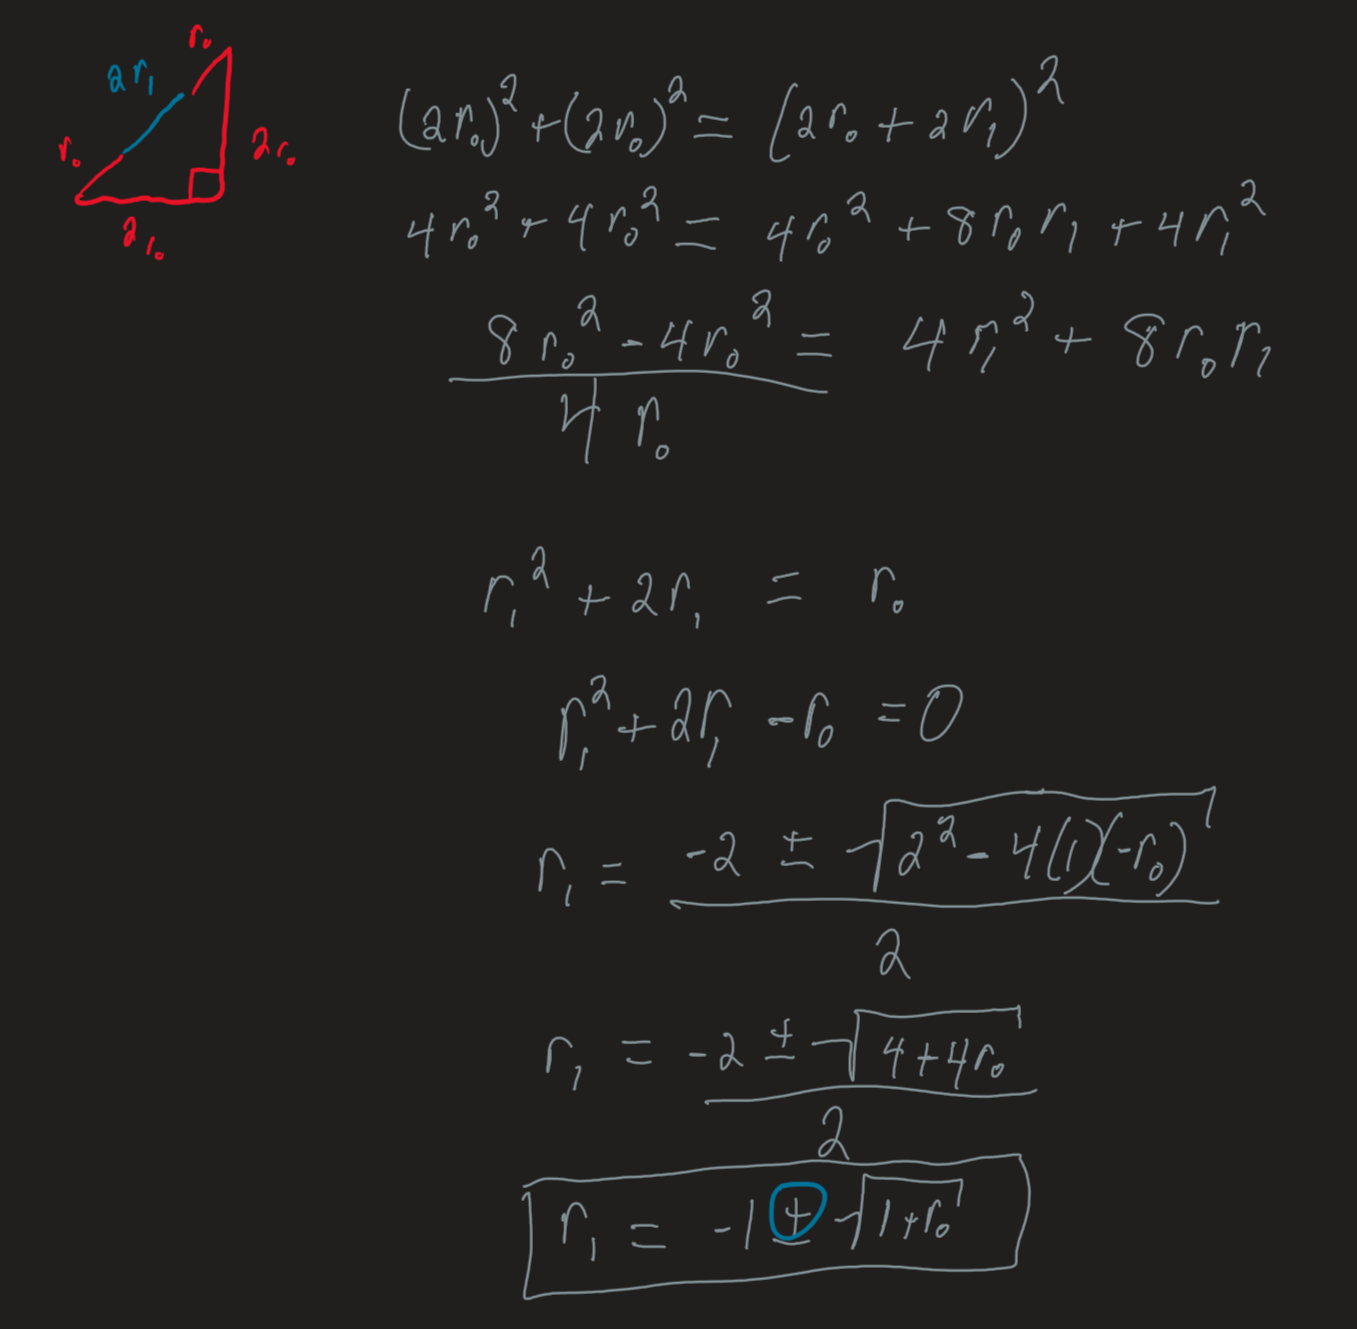
\includegraphics[width=0.7\textwidth]{fig/pblm4b_1.png}
\end{figure}
thus $r_1 \leq -1 + \sqrt{1 + r_0}$.\\
This is then proven as countable by the same logic as $A_0^*$.\\
Additionally, this process can be repeated for more collections of disks of decreasing size 
until $r_i$ is infinitey small.\\
At first glance the union of all these sets may not actually be proven to be coundable, 
but each additional set will no longer consist of all potential optimal pairs so it 
may be possible to limit this to $\aleph_0$



\newpage
\subsection{Any collection of non-intersecting T-shapes on a plane}
\textbf{Note:} T-shape consists of two perpendicular line segments such that 
one of the segments is attached by one of its endpoints to the center of the other segment. 
The lengths of these segments can be arbitrary. The orientation of the T-shape can be arbitrary.\\

Define set $A$,
\begin{align*}
	A := &\Bigg{\{}
		((x_1,y_1),(x_2,y_2),(x_3,y_3)) \in (\R^2)^3: \\
		&\quad\forall \qty((x_1^{(i)},y_1^{(i)}),(x_2^{(i)},y_2^{(i)}),(x_3^{(i)},y_3^{(i)})) \in (\R^2)^3\\ 
		&\quad ((x_1,y_1)\Rel(x_2,y_2) \cap ((x_1^{(i)},y_1^{(i)})\Rel)(x_2^{(i)},y_2^{(i)}) = \emptyset)\\
		&\quad \land \qty((\cfrac{x_1+x_2}{2},\cfrac{y_1+y_2}{c})\Rel(x_3,y_3)) 
			\cap \qty(\cfrac{x_1^{(i)}+x_2^{(i)}}{2},\cfrac{y_1^{(i)}+y_2^{(i)}}{c}) = \emptyset)
	\Bigg{\}}
\end{align*}
with $\Rel$ defined as
\begin{displaymath}
	\Rel := \qty{
		(x,y) \in \R \cross \R, \ t \in \R : 
		(x = (1-t) x_a + t x_b) \land (y = (1-t) y_a + t y_b)
		\land (0 \leq t \leq 1)
	}
\end{displaymath}


Let arbritrary parameters $l_1, l_2$ be used to define the set $A$,
\begin{displaymath}
	A := \qty{((x_1,y_1),(x_2,y_2),(x_3,y_4)) \in (\R^2)^3 :}
\end{displaymath}


% do more here....











\subsection{Set $\mathbb{P}$ of all prime numbers}
By definition, all prime numbers are natural numbers, thus
\begin{displaymath}
	\mathbb{P} \subseteq \N
\end{displaymath}
This then implies that $\abs*{\mathbb{P}} \leq \abs*{\N}$, therefore $\mathbb{P}$ is countable.
\begin{displaymath}
	\mathbb{P} \subseteq \N \implies \abs*{\mathbb{P}} \leq \abs*{\N}
\end{displaymath}


\subsection{Set $\mathbb{A}$ of all algebraic numbers}
\textbf{Note:} Algebraic numbers are numbers which are roots of 
some polynomials with integer coefficients.









\newpage
% Problem 5
\section{}
Prove that for any infinite set $A$ there exists $B \subseteq A$, so that $\abs{B}=\abs{\N}$.\\

By definition an infinite set, $\abs*{A} \geq \abs{\N} = \aleph_0$.
A very, very simple proof of the fact $\exists B \subseteq A : \abs{B}=\abs{\N} = \aleph_0$ 
is as follows:

Define $f : \N \toB B$ (bijective) to directly map $\N$ to an element of subset $B$. 
Since $f$ is bijective, $\abs{B}=\abs{\N} = \aleph_0$.\\
Next, define $g : B \toI A$ (injective). Becouse $A$ is an infinite set, 
and injective function $g$ can in fact map the infinite set $B$ into $A$, 
which then implies $B \subseteq A$.

\begin{displaymath}
	(f : \N \toB B) \land (g : B \toI A) \implies \abs*{A} \geq \abs*{B} = \abs*{\N} = \aleph_0
\end{displaymath}


\newpage
% Problem 6
\section{}
Prove that the following sets have the same cardinality.
\begin{figure}[h]
	\centering
	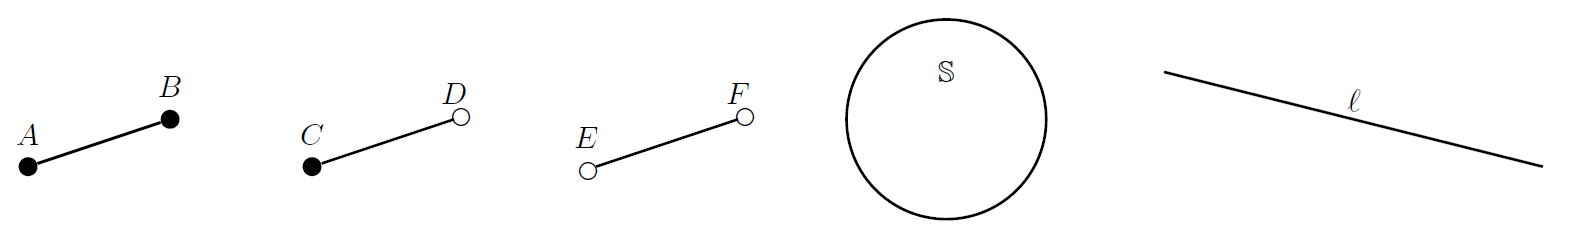
\includegraphics[width=\textwidth]{fig/pblm6.png}
\end{figure}

These sets can all be represented as a set of real number ordered pairs.\\
These are constructed with arbritrary constants: 
$x_a,x_b,x_c,x_d,x_e,x_f,y_a,y_b,y_c,y_d,y_e,y_f,x_s,y_s,r_s,m_l,b_l$

\begin{align*}
	AB &= \{(x,y) \in \R^2, \ t \in \R : 
	(x = (1-t) x_a + t x_b) \land (y = (1-t) y_a + t y_b)
	\land (0 \leq t \leq 1)\}\\
	CD &= \{(x,y) \in \R^2, \ t \in \R : 
	(x = (1-t) x_c + t x_d) \land (y = (1-t) y_c + t y_d)
	\land (0 \leq t < 1)\}\\
	EF &= \{(x,y) \in \R^2, \ t \in \R : 
	(x = (1-t) x_e + t x_f) \land (y = (1-t) y_e + t y_f)
	\land (0 < t < 1)\}\\
	\mathbb{S} &= \{(x,y) \in \R^2, \ t \in \R : 
	(x = r_s cos(2 \pi t) + x_s) \land (y = sin(2 \pi t) + y_s)
	\land (0 \leq t < 1)\}\\
	\mathit{l} &= \{(x,y) \in \R^2, \ t \in \R: (x = t) \land (y = m_l t + b_l)\}
\end{align*}

It is clear that each set is defined parmetrically with bijective equations maping 
the parameter $t$ into a 2-D corndates $(x,y)$, thus proving that the cardinality 
of each sets parameter is sufficent to showing the each set has the same cardinality.\\

Let $T_i = \{t \in A_i\}$ for each of the sets $A_i$, then (from the reasoning above) 
the following can be said:

\begin{align*}
	T_{AB} &= \{t \in \R : 0 \leq t \leq 1\}, \ &\abs{T_{AB}} = \abs{AB}\\
	T_{CD} &= \{t \in \R : 0 \leq t < 1\}, \ &\abs{T_{CD}} = \abs{CD}\\
	T_{EF} &= \{t \in \R : 0 < t < 1\}, \ &\abs{T_{EF}} = \abs{EF}\\
	T_{\mathbb{S}} &= \{t \in \R : 0 \leq t < 1\}, \ &\abs{T_{\mathbb{S}}} = \abs{\mathbb{S}}\\
	T_{\mathit{l}} &= \{t \in \R\}, \ &\abs{T_{\mathit{l}}} = \abs{\mathit{l}}\\
\end{align*}

Clearly, the equivalent definition of $T_{CD}$ and $T_{\mathbb{S}}$ indicates
$$\abs*{CD} = \abs*{T_CD} = \abs*{T_\mathbb{S}} = \abs*{\mathbb{S}}$$

The equivalence of the other sets is more difficult then via definition.\\
First, the baseline cardinality can be shown to be $\aleph_1$ as (by definition of $T_{\mathit{l}})$)
$$\abs{T_\mathit{l}} = \abs{\R} = \aleph_1$$

Next, the equivalence of $T_{EF}$ and $T_\mathit{l}$ can be shown with the biforjective mapping 
$$f_1 : \R \rightarrow T_{EF} = \frac{2 \pi \tan^{-1}(x) + 1}{2}$$
Therefore,
$$\abs{EF} = \abs{T_{EF}} = \abs{T_{\mathit{l}}} = \abs{\R} = \aleph_1$$

Next, due to the nature of infinite sets, the addition of $t=0$ from $T_{EF}$ to $T_{CD}$ 
does not affect the overall cardinality of $T_{CD}$, thus
$$\abs{CD} = \abs{T_{CD}} = \abs{T_{EF}} = \abs{\R} = \aleph_1$$

Similarly, the addition of $t=1$ from $T_{CD}$ to $T_{AB}$ will stil result in 
$$\abs{AB} = \abs{T_{AB}} = \abs{T_{CD}} = \abs{\R} = \aleph_1$$

Ultimently this means that
$$\abs{AB} = \abs{CD} = \abs{EF} = \abs{\mathbb{S}} = \abs{\mathit{l}} = \abs{\R} = \aleph_1$$



\end{document}
